\documentclass{standalone}
\usepackage{tikz}

\begin{document}
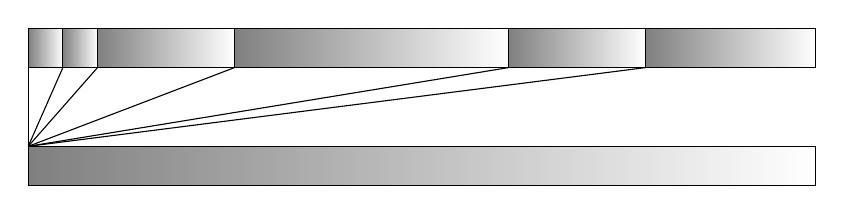
\begin{tikzpicture}

% \draw[help lines, color=gray!30] (-1,-20) grid (50,20);

\tikzstyle{every path}=[draw] % all paths are drawn
% \fill (0,0) rectangle +(1,1);
\shade [shading=axis,shading angle=90](0,0) rectangle +(0.44,.5);
\shade [shading=axis,shading angle=90](0.44,0) rectangle +(0.44,.5);
\shade [shading=axis,shading angle=90](0.88,0) rectangle +(1.74,.5);
\shade [shading=axis,shading angle=90](2.62,0) rectangle +(3.48,.5);
\shade [shading=axis,shading angle=90](6.1,0) rectangle +(1.74,.5);
\shade [shading=axis,shading angle=90](7.84,0) rectangle +(2.16,.5);

% Quant = 0
\shade [shading=axis,shading angle=90](0,-1.5) rectangle +(10,.5);
\draw[] (0,0) -- (0,-1);
\draw[] (0.44,0) -- (0,-1);
\draw[] (0.88,0) -- (0,-1);
\draw[] (2.62,0) -- (0,-1);
\draw[] (6.1,0) -- (0,-1);
\draw[] (7.84,0) -- (0,-1);


% \node (a) {A} node (b) at (0.5,1.5) {0.1} node (c) at (2,-1) {C};


\end{tikzpicture}
\end{document}